\chapter{Unsupervised Learning}
\label{sec:unsupervised-learning}
Unsupervised learning attempts to learn from data without supplied task labels.
The choice of objective determines what the algorithm considers meaningful.
The main possibilities are: 
\begin{itemize}
    \item \textbf{Clustering} which observations belong together?,
    \item  \textbf{Density Estimation} where is probability mass?,
    \item \textbf{Latent Structure} can fewer factors explain the data?, and 
    \item \textbf{Anomaly Detection} which observations are unusual?.
\end{itemize}

\begin{figure}[htbp]
    \centering
    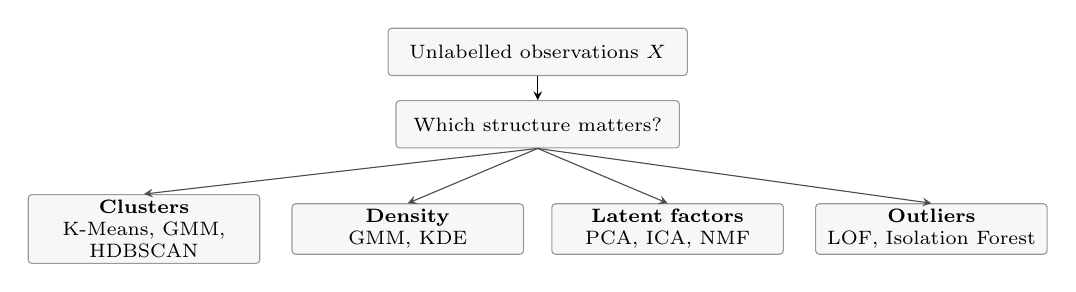
\begin{tikzpicture}[font=\scriptsize, >=stealth, node distance=3mm]
         \tikzset{ulbox/.style={draw=black!40,rounded corners=1.3pt,fill=black!3,align=center,minimum height=6mm,inner sep=2pt}}
         \node[ulbox,minimum width=38mm] (x) at (0,1.45) {Unlabelled observations $X$};
         \node[ulbox,minimum width=36mm] (q) at (0,.53) {Which structure matters?};
         \draw[->] (x)--(q);
         \node[ulbox,text width=28mm] (c) at (-5,-.8) {\textbf{Clusters}\\K-Means, GMM, HDBSCAN};
         \node[ulbox,text width=28mm] (d) at (-1.65,-.8) {\textbf{Density}\\GMM, KDE};
         \node[ulbox,text width=28mm] (l) at (1.65,-.8) {\textbf{Latent factors}\\PCA, ICA, NMF};
         \node[ulbox,text width=28mm] (a) at (5,-.8) {\textbf{Outliers}\\LOF, Isolation Forest};
         \foreach \n in {c,d,l,a}{\draw[->,black!70] (q.south) -- (\n.north);}
    \end{tikzpicture}
    \caption{Unsupervised learning taxonomy.}
    \label{fig:taxonomy}
\end{figure}


\section{Representation Similarity}
\label{sec:Representation Similarity foundations}
A cluster is a statement about \emph{representation similarity}, not a property of raw data alone.
Non-data based effects like representation choice and similarity metric choice decide clusters just as much as the raw data.
For observations $X\in\mathbb R^{N_{\text{samples}}\times N_{\text{features}}}$, changing representations (units, irrelevant features or standardisation) can change clusters.
And, for similarity metrics, we have many options
\begin{itemize}
    \item \textbf{Euclidean} distance preserves raw differences,
    \item \textbf{Cosine} compares direction rather than magnitude, 
    \item \textbf{Mahalanobis} measures separation after accounting for a chosen covariance geometry.
\end{itemize}

\begin{calloutmemoryhook}
    Clustering discovers structure between representations you choose in the distance metric you chose.
\end{calloutmemoryhook}


\begin{center}
    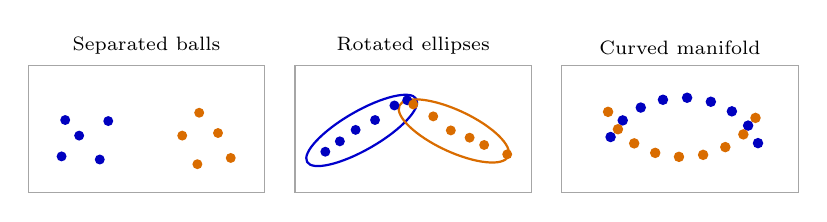
\begin{tikzpicture}[font=\scriptsize,x=.77cm,y=.66cm]
     \foreach \s/\name in {0/{Separated balls},4.4/{Rotated ellipses},8.8/{Curved manifold}} {
       \begin{scope}[shift={(\s,0)}]
        \draw[black!35] (0,0) rectangle (3.9,2.45);
        \node[anchor=south] at (1.95,2.48) {\name};
       \end{scope}
     }
     \foreach \x/\y in {.55/.7,.84/1.10,1.18/.64,.61/1.40,1.32/1.38,2.54/1.1,2.82/1.54,3.13/1.15,2.79/.55,3.34/.67}{\ifdim\x pt<2pt \fill[blue!75!black](\x,\y) circle(1.8pt); \else \fill[orange!85!black](\x,\y) circle(1.8pt);\fi}
     \begin{scope}[shift={(4.4,0)}]
      \draw[blue!80!black,thick,rotate around={30:(1.1,1.2)}] (1.1,1.2) ellipse (1.04 and .37);
      \draw[orange!85!black,thick,rotate around={-25:(2.62,1.19)}] (2.62,1.19) ellipse (.99 and .4);
      \foreach \x/\y in {.5/.79,.74/.99,1/1.21,1.32/1.4,1.64/1.68,1.85/1.78}{\fill[blue!75!black](\x,\y) circle(1.8pt);}
      \foreach \x/\y in {1.95/1.7,2.28/1.47,2.57/1.2,2.88/1.06,3.12/.92,3.5/.74}{\fill[orange!85!black](\x,\y) circle(1.8pt);}
     \end{scope}
     \begin{scope}[shift={(8.8,0)}]
       \foreach \a in {15,33,51,69,87,105,123,141,159}{\fill[blue!75!black] ({2+1.28*cos(\a)},{.65+1.18*sin(\a)}) circle (1.9pt);}
       \foreach \a in {195,213,231,249,267,285,303,321,339}{\fill[orange!85!black] ({2+1.28*cos(\a)},{1.86+1.17*sin(\a)}) circle (1.9pt);}
     \end{scope}
    \end{tikzpicture}
    \caption{Same two-colour objective, three geometries: centroids suit compact balls, covariance models tilted ellipses, and density/graph connections can represent curved groups.}
    \label{fig:geometries}
\end{center}

\section{Centroid Clustering}
\label{sec:kmeans}
\paragraph{K-Means} alternates two operations.
\begin{enumerate}
    \item assign every observation to its nearest \textbf{centroid},
    \item then \textbf{move} each centroid to the mean of its assigned observations.
\end{enumerate}
These operations preserve the within-cluster squared Euclidean error, so the algorithm converges to a local optimum, not necessarily the global one.
\[
    \underbrace{\min_{\{\mu_k\},\{c_i\}}\sum_{i=1}^{N_{\text{samples}}}\|x_i-\mu_{c_i}\|_2^2}_{\text{within-cluster squared distance}}
    \qquad\Longleftrightarrow\qquad
    \underbrace{c_i\gets\arg\min_k\|x_i-\mu_k\|_2^2}_{\text{assign}}
    \ \to\ 
    \underbrace{\mu_k\gets\operatorname{mean}_{i:c_i=k}(x_i)}_{\text{recentre}}.
\]

\paragraph{K-Means++} seeds centroids to spread them across the data, reducing poor initialisations.
Multiple seeds still matter because the objective is non-convex.
\paragraph{Mini-Batch K-Means} estimates centroid updates from subsets and therefore scales better to large datasets, at the cost of noisier, potentially less accurate solutions.
\paragraph{K-Medoids} uses actual observations as representatives and can use non-Euclidean dissimilarities.
It is less sensitive to extreme values than means, but often costs more to fit.

The basic iteration costs roughly $O(N_{\text{samples}}K N_{\text{features}})$ per pass, so the number of iterations and repeats determine the actual work needed.
Because errors are squared, a distant outlier can pull a mean markedly, and K-Means must assign that outlier to some cluster even when no group is credible.
Increasing $N_{\text{Clusters}}$ can reduce within-cluster error simply by spending more centroids, so a lower objective value does not by itself establish a more meaningful partition.


\begin{figure}[htbp]
    \centering
    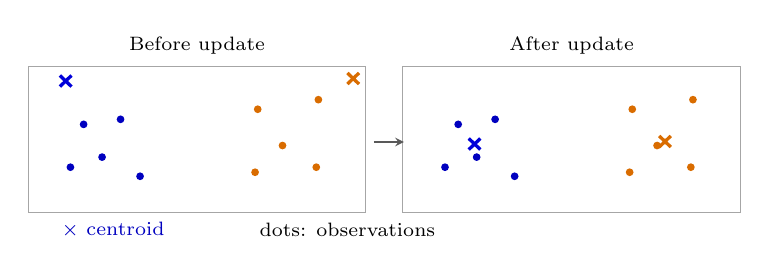
\begin{tikzpicture}[x=.67cm,y=.64cm,font=\scriptsize,>=stealth]
        \foreach \shift/\lab in {0/{Before update},7.1/{After update}}{
            \begin{scope}[shift={(\shift,0)}]
                \draw[black!35] (-.2,-.2) rectangle (6.2,2.7);
                \foreach \px/\py in {.6/.7,1.2/.9,.85/1.55,1.55/1.65,1.92/.52,4.1/.6,4.62/1.13,5.26/.7,4.15/1.85,5.3/2.04}{
                    \ifdim\px pt<3pt
                        \fill[blue!75!black] (\px,\py) circle (1.4pt);
                    \else
                        \fill[orange!85!black] (\px,\py) circle (1.4pt);
                    \fi
                }
                \node[anchor=south] at (3,2.75) {\lab};
            \end{scope}
        }
        \draw[blue!85!black,very thick] (.4,2.3)--(.62,2.52) (.4,2.52)--(.62,2.3);
        \draw[orange!85!black,very thick] (5.85,2.35)--(6.07,2.57) (5.85,2.57)--(6.07,2.35);
        \draw[blue!85!black,very thick] (8.15,1.05)--(8.37,1.27) (8.15,1.27)--(8.37,1.05);
        \draw[orange!85!black,very thick] (11.76,1.1)--(11.98,1.32) (11.76,1.32)--(11.98,1.1);
        \draw[->,black!65] (6.35,1.2)--(6.92,1.2);
        \node[blue!75!black,anchor=west] at (.25,-.55) {$\times$ centroid};
        \node[anchor=west] at (4.0,-.55) {dots: observations};
    \end{tikzpicture}
    \caption{K-Means updates centroids after nearest-centre assignments.}
    \label{fig:kmeans}
\end{figure}

\begin{calloutpractical}
    If groups are circular, nearest-centroid partitions are effective; elongated, curved, unequal-density or overlapping groups violate this bias.    
\end{calloutpractical}


\section{Probabilistic Clustering}
\label{sec:gmm}
\paragraph{Gaussian Mixture Model (GMM)}
Gaussian Mixture Models (GMM) work by dropping independent Gaussian distributions on the feature space and moving them (shifting mean and standard deviations) until they represent the clusters well.
because of the probability nature of these distributions, observations can have \emph{partial membership} in several groups.
The weighted components also define a probability density.
Unlike K-Means, GMM can model substantial overlap.
A fitted Gaussian component does not correspond to a meaningful physical class.
\[
    \underbrace{p(x)}_{\text{mixture density}}
    =\sum_{k=1}^{K}\underbrace{\pi_k}_{\text{component prevalence}}
    \underbrace{\mathcal N(x\mid\mu_k,\Sigma_k)}_{\text{component shape}},
    \quad \sum_k\pi_k=1;
    \qquad
    \underbrace{P(c_i=k\mid x_i)}_{\text{soft membership}}
    =\frac{\pi_k\mathcal N(x_i\mid\mu_k,\Sigma_k)}{\sum_j\pi_j\mathcal N(x_i\mid\mu_j,\Sigma_j)}.
\]
\paragraph{Expectation-Maximisation (EM)} is the optimisation process. 
It alternates between estimating how much each component explains every observation (E-step) and refitting component parameters using those fractional memberships (M-step).
Each exact EM iteration does not decrease the observed-data likelihood, but can converge to a poor local optimum.
The M-step provides a new mean and covariance,
\[
    \underbrace{\mu_k\gets\frac{\sum_i r_{ik}x_i}{\sum_i r_{ik}}}_{\text{membership-weighted centre}},\qquad
    \underbrace{\pi_k\gets\frac{\sum_i r_{ik}}{N_{\text{samples}}}}_{\text{component prevalence}},\qquad
    \underbrace{\Sigma_k\gets\frac{\sum_i r_{ik}(x_i-\mu_k)(x_i-\mu_k)^\top}{\sum_i r_{ik}}}_{\text{within-component covariance}},
\]
with $r_{ik}=P(c_i=k\mid x_i)$ from the E-step.
A point lying equally between two components has values near $(0.5,0.5)$, while a distant well-separated point tends towards a near-binary assignment.
This fractional accounting is the main difference from K-Means.


\subsection{Covariance}
\begin{itemize}
    \item \textbf{Spherical} covariance assumes equally shaped balls, 
    \item \textbf{Diagonal} covariance permits axis-aligned ellipses, 
    \item \textbf{Full} covariance permits rotated ellipses.
    It costs $O(KN_{\text{features}}^2)$ parameters and can overfit, 
    \item \textbf{Tied} covariance shares a shape across components.
\end{itemize}

\begin{calloutpractical}
    Choose $N_{\text{Clusters}}$ using held-out likelihood or complexity-aware criteria such as BIC as a density-model baseline, and separately test whether the assignments are stable and useful.    
\end{calloutpractical}

\begin{calloutspecialcase}
    With equal spherical covariances and vanishing variance, the dominant GMM component becomes the nearest mean.
    Hard assignments approach K-Means (under the corresponding objective assumptions).
\end{calloutspecialcase}

\begin{calloutmemoryhook}
    K-Means assigns a centre, and GMM assigns a probability distribution.
\end{calloutmemoryhook}

\section{Hierarchical clustering}
\label{sec:hierarchical}
\paragraph{Agglomerative Hierarchical Clustering} starts with one cluster per observation and repeatedly merges the closest pair of clusters.
It produces a \textbf{dendrogram} (think; tree roots), where the height of each merge records the chosen dissimilarity, and cutting the tree at different heights changes the clustering resolution without rerunning the merges.
The meaning of ``closest'' is set by \textbf{linkage}: 
\begin{itemize}
    \item \textbf{Single:} nearest pair (can chain via bridges), 
    \item \textbf{Complete:} farthest pair (favour compact groups), 
    \item \textbf{Average:}  mean pairwise distance, 
    \item \textbf{Ward:} smallest increase in within-cluster squared error (normally Euclidean).
\end{itemize}

Agglomerative methods avoid a single pre-specified $N_{\text{Clusters}}$ and expose nested structure, which is great for developers.
However, early incorrect merges cannot be undone.
Naive implementations require quadratic distance storage, often limiting use on very large datasets.
\paragraph{Divisive} hierarchical clustering reverses the construction (start with one cluster, recursively split), but is less commonly used.

\begin{center}
    \begin{minipage}{\linewidth}\centering
    \begin{tikzpicture}[x=.75cm,y=.50cm,font=\scriptsize,thick]
         \foreach \x/\lbl in {0/A,1/B,2/C,3/D,4/E,5/F}{\node at (\x,-.38) {\lbl};}
         \draw (0,0)--(0,1) --(1,1)--(1,0);
         \draw (.5,1)--(.5,2.7)--(2.5,2.7)--(2.5,1.35);
         \draw (2,0)--(2,1.35)--(3,1.35)--(3,0);
         \draw (4,0)--(4,.78)--(5,.78)--(5,0);
         \draw (4.5,.78)--(4.5,3.35)--(1.5,3.35)--(1.5,2.7);
         \draw[densely dashed,blue!70] (-.35,1.95)--(5.35,1.95);
         \node[anchor=west] at (5.55,1.95) {cut height};
         \node[anchor=east,rotate=90] at (-.50,1.55) {merge distance};
         \caption{The dendrogram preserves nested merges; changing the cut produces a different number of groups.}
    \end{tikzpicture}
    \label{fig:dendrogram}
    \end{minipage}
\end{center}


\section{Density Clustering}
\label{sec:density-clustering}
\paragraph{DBSCAN} defines a neighbourhood of radius $\varepsilon$ around each observation and marks a point as a \textbf{core} when it has at least $N_{\text{min points}}$ observations in that neighbourhood (typically counting itself).
Each datapoint within the radius is like a distance weighted vote on the density, generating clean transitions even where datapoints are sparse.
Connected core regions become clusters, nearby non-core points may be included as \textbf{border} points, and unassigned observations are \textbf{noise}.
It can find curved, irregular groups and reject isolated observations without choosing $N_{\text{Clusters}}$.
However, one global $\varepsilon$ struggles when meaningful groups have different densities, because a radius that merges a sparse group may also merge nearby dense groups.

\begin{center}
    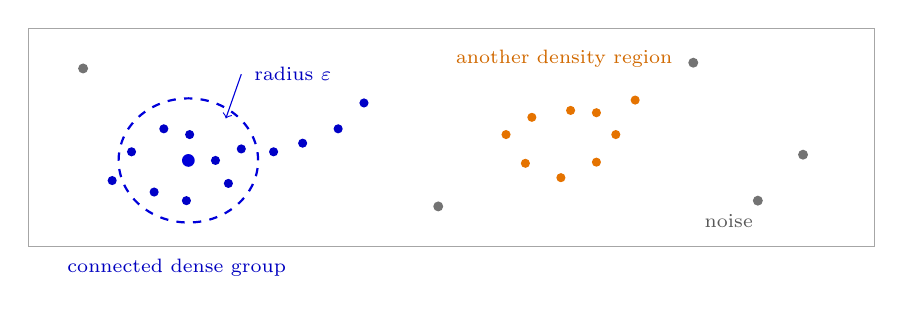
\begin{tikzpicture}[x=.82cm,y=.73cm,font=\scriptsize]
     \draw[black!35] (-.3,-.25) rectangle (12.8,3.55);
     \foreach \x/\y in {1/.9,1.3/1.4,1.8/1.8,2.2/1.7,2.6/1.25,2.8/.85,1.65/.70,2.15/.55,3/1.45,3.5/1.4,3.95/1.55,4.5/1.8,4.9/2.25}{\fill[blue!78!black] (\x,\y) circle (1.65pt);}
     \foreach \x/\y in {7.1/1.7,7.5/2.0,8.1/2.12,8.5/2.08,8.8/1.70,8.5/1.22,7.95/.95,7.4/1.2,9.1/2.3}{\fill[orange!90!black] (\x,\y) circle (1.65pt);}
     \foreach \x/\y in {.55/2.85,6.05/.45,10/2.95,11.7/1.35,11/0.55}{\fill[black!55] (\x,\y) circle (1.8pt);}
     \draw[blue!85!black,dashed,thick] (2.18,1.25) circle (1.08);
     \fill[blue!85!black] (2.18,1.25) circle (2.3pt);
     \draw[->,blue!85!black] (3.0,2.75)--(2.76,1.98);
     \node[anchor=west,blue!75!black] at (3.05,2.76) {radius $\varepsilon$};
     \node[blue!75!black] at (2,-.62) {connected dense group};
     \node[orange!82!black] at (8,3.02) {another density region};
     \node[black!65] at (10.55,.20) {noise};
    \end{tikzpicture}
    \caption{DBSCAN grows groups through core-point density connectivity, while leaving sufficiently isolated observations unassigned.}\label{fig:dbscan}
\end{center}

\paragraph{HDBSCAN} extends the density approach by constructing a hierarchy using density-sensitive (mutual-reachability) distances, then selecting clusters that persist over a range of density levels.
Its main practical controls are minimum cluster size and minimum samples.
Minimum size encodes how small a group is worth retaining, while increasing minimum samples usually makes the selection more conservative.
Smaller minimum cluster size admits more fine-grained groups but may label sampling fluctuations as discoveries.
Larger values favour coarser, more persistent structures.
A returned membership strength reflects the algorithm's notion of cluster persistence, not a calibrated posterior probability that the physical state is ``correct''.
Unlike DBSCAN, a single $\varepsilon$ is not the main global cut, though severe density variation and a poorly chosen representation remain problematic.
\paragraph{OPTICS} orders observations to reveal density-connected structure over several neighbourhood scales.
Generally, it's useful when a single DBSCAN radius is insufficient and a density ordering is itself informative.


\section{Spectral Clustering}
\textbf{Spectral Clustering} changes the problem from clustering points by their coordinates to clustering a graph by its connectivity.
Build a graph ($W_{ij}$) by joining observations (nodes) by their similarity (edges).
The graph may be fully connected, $\epsilon$-neighbourhood, or $k$-nearest-neighbour.
Sparse neighbour graphs avoid storing every pairwise connection.
The diagonal \textbf{degree matrix} stores each node's total connection strength by summing all its connections.
A \textbf{graph Laplacian} then compares this total connectivity with the individual connections in $W$, with many possible methods:
\begin{itemize}
    \item \textbf{Unnormalised:} $L=D-W$.
    \item \textbf{Symmetric normalised:} $L_{\mathrm{sym}}=I-D^{-1/2}WD^{-1/2}$.
    \item \textbf{Random-walk normalised:} $L_{\mathrm{rw}}=I-D^{-1}W$.
\end{itemize}

Take the smallest eigenvalued eigenvectors and stack them as
\[
    U\in\mathbb{R}^{N_{\mathrm{points}}\times N_{\mathrm{clusters}}}.
\]
Each row of $U$ is the original point expressed in graph-connectivity coordinates rather than feature coordinates.
Disconnected graph components give zero eigenvalues and weakly connected groups give corresponding low-eigenvalue directions.
For $L_{\mathrm{sym}}$, the rows of $U$ are commonly normalised before running K-Means on these new coordinates.

\begin{calloutintuition}
    In summary, make a similarity matrix and make a low rank reduction of it, and then do usual clustering methods on it.
\end{calloutintuition}

\begin{calloutpractical}
    For strong inter-cluster and weak intra-cluster connectivity, spectral clustering can recover non-convex groups that centroid methods miss.
\end{calloutpractical}

\begin{calloutpractical}
    The main choices are how similarity is defined, which edges are kept, which Laplacian is used, and how many eigenvectors/clusters are retained.
    Spectral clustering gains flexible cluster geometry, but building and eigendecomposing the similarity graph becomes expensive for large datasets.
\end{calloutpractical}

\section{Kernel Density Estimation (KDE)}
KDE places a smooth kernel at each observation and adds these contributions to estimate the full density without first assuming $N_{\text{Clusters}}$ Gaussian components.
For an isotropic kernel in $N_{\text{features}}$ dimensions, $\hat p(x)\propto \sum_i K((x-x_i)/h)/(N_{\text{samples}}h^{N_{\text{features}}})$; \textbf{bandwidth $h$} is the main smoothness choice.
Small $h$ gives a spiky density and large $h$ merges local structure; density estimation becomes substantially harder as dimensions increase, and naive query cost scales with the number of observations.

\section{Latent Factorisation}
\textbf{PCA} extracts orthogonal maximum-variance directions; the existing \emph{Data: Preprocessing} section already explains its eigenvector and whitening views.
\textbf{Independent Component Analysis (ICA)} seeks statistically independent sources rather than merely uncorrelated directions, typically relying on non-Gaussian independent components and an identifiable mixing model.
\textbf{Non-negative Matrix Factorisation (NMF)} approximates a non-negative data matrix as two non-negative factors, $X\approx WH$, encouraging additive, parts-based explanations; the components are generally not unique.
For neural nonlinear compression, see autoencoders in \emph{Model Family Overview} and VAEs in \emph{Generative Modelling}; neither reconstruction loss nor a smooth latent plot guarantees clusters useful for a downstream task.

\begin{center}
\begingroup\ULtight\small
\begin{tabular}{@{}p{.16\linewidth}p{.30\linewidth}p{.30\linewidth}p{.17\linewidth}@{}}
\hline
\textbf{Method} & \textbf{Assumption / structure} & \textbf{Use when} & \textbf{Main limitation}\\\hline
K-Means & Compact groups around means & Cheap flat partition of many points & Hard, nearly spherical groups\\
GMM / EM & Mixture of Gaussian densities & Overlap, uncertainty, density needed & Covariance and likelihood fragility\\
Hierarchical & Groups have useful nested merges & Explore scale and linkage & Cost; merges irreversible\\
DBSCAN & Dense connected sets + noise & Irregular shapes, explicit noise & Global density threshold\\
HDBSCAN & Stable density hierarchy & Density varies; abstention useful & Sensitivity to sampling/geometry\\
Spectral & Similarity graph has weak cuts & Manifold / graph-separated groups & Graph build and eigensolver\\
KDE & Smooth sum of local kernels & Low-dim density estimation & Bandwidth; high-dimensional cost\\
ICA / NMF & Independent sources / additive factors & Interpretable latent decomposition & Strong assumptions; ambiguity\\\hline
\end{tabular}
\ULtabcap{Primary inductive biases and decision boundaries; these algorithms answer different questions rather than forming a single ranking.}\label{tab:family}
\endgroup
\end{center}

\section{Anomaly detection without anomaly labels}\label{sec:anomaly}
An \textbf{anomaly score} ranks how unusual an observation is relative to the training distribution; it does not establish that the observation is faulty, harmful or causally exceptional.
A physical fault may occur in a dense region, while a legitimate new operating regime may appear as an isolated point.
\textbf{Isolation Forest} builds random partition trees and scores observations by how quickly they become isolated: unusual points tend to require fewer splits.
\textbf{Local Outlier Factor (LOF)} compares local density with nearby neighbours, identifying points that are sparse \emph{relative to their surroundings}; its neighbour count determines the scale of abnormality.
\textbf{GMM/KDE likelihood} can rank low-density points, but likelihood is not automatically a reliable anomaly score in high dimensions: density depends on representation/units, and high-likelihood regions need not match the distribution's typical set.
Autoencoder reconstruction error is another option; a high-capacity decoder can reconstruct some anomalous samples well and fail on legitimate but rare ones.

\begin{calloutmemoryhook}
Unusual under a model is not necessarily wrong in the world.
\end{calloutmemoryhook}
\subsection{Deployment threshold.}
If a review team can investigate only $B$ items per day, choose the top-$B$ scores or calibrate a threshold against a labelled review set or a representative reference period.
State the expected alert rate, missed-event cost and sensitivity to drift; do not describe a nominal contamination fraction as a known real-world fault prevalence.
The same evaluation problem occurs in \emph{Use Case: Real-Time Moderation}, where ranking, threshold and review capacity are separate design decisions.

\section{Evaluation: when there is no correct label}\label{sec:evaluation}
An internal clustering score measures whether the algorithm satisfies a geometric criterion, not whether the resulting groups correspond to meaningful physics or useful decisions.
The evaluation must distinguish \textbf{geometric fit}, \textbf{stability}, and \textbf{downstream value}.
\begin{center}
\begingroup\ULtight\small
\begin{tabular}{@{}p{.20\linewidth}p{.36\linewidth}p{.35\linewidth}@{}}
\hline
\textbf{Measure} & \textbf{What it rewards} & \textbf{Why it can mislead}\\\hline
Silhouette & Tight points separated from next-nearest cluster; $s_i=(b_i-a_i)/\max(a_i,b_i)$ & Prefers particular distance geometry; irregular dense groups may score poorly\\
Davies--Bouldin & Low within-group scatter compared with inter-centre separation (lower is better) & Inherits centroid/compactness assumptions\\
Log-likelihood & High probability assigned by density model to held-out data & High density is not semantic membership or guaranteed OOD detection\\
AIC / BIC & Likelihood balanced against model parameter count & Approximate selection assumptions; best density fit may not give best groups\\
Stability / ARI & Similar assignments under sampling, seeds or perturbations & A stable answer can still be arbitrary or irrelevant\\
Downstream utility & Improvement on retrieval, forecasting, fault detection, scientific discovery & Needs a well-designed external task; may leak labels into selection\\\hline
\end{tabular}
\ULtabcap{Evaluation criteria test different desiderata; no universal unsupervised score is a substitute for task validation.}\label{tab:metrics}
\endgroup
\end{center}

\subsection{Failure diagnostics.}
The most useful next step is usually a controlled intervention on the representation or the model assumption, not a more complicated algorithm.
\begin{center}
\begingroup\ULtight\small
\begin{tabular}{@{}p{.32\linewidth}p{.32\linewidth}p{.29\linewidth}@{}}
\hline
\textbf{Observed behaviour} & \textbf{Possible mechanism} & \textbf{Next experiment}\\\hline
Clusters change after feature scaling & A few units/features dominate distance & Inspect feature contribution; standardise or weight deliberately\\
K-Means gives one huge, one tiny group & Unequal density, outliers or poor $N_{\text{Clusters}}$ & Check seeds; try GMM or density clustering\\
GMM covariance nearly singular & Component fits one/few observations & Regularise; reduce dimension; compare covariance type\\
DBSCAN: nearly everything is noise & Neighbourhood too small for the sampling density & Revisit $\varepsilon$, min points and representation\\
Single linkage forms a long chain & Thin bridges connect distant groups & Compare average/complete/Ward linkage\\
Clusters align with collection date & Instrument or acquisition batch shift & Hold out dates/apparatus; inspect raw features\\
Only t-SNE produces separated islands & Projection exaggerates local gaps & Quantify clusters in the original embedding\\
\hline
\end{tabular}
\ULtabcap{Failure modes should trigger experiments that distinguish representation errors from algorithm assumptions.}\label{tab:failures}
\endgroup
\end{center}

\subsection{Internal geometry.}
In the silhouette expression, $a_i$ is an observation's average distance to its assigned cluster and $b_i$ the smallest average distance to another cluster.
A score near $1$ reflects separation under that distance, near $0$ an ambiguous boundary; it does not imply true discrete categories.
The elbow of K-Means inertia against $N_{\text{Clusters}}$ is only a heuristic: the cost always decreases or stays fixed as $N_{\text{Clusters}}$ increases, often without a distinct bend.
\subsection{Stability.}
Repeat fitted pipelines across seeds and bootstrap or subsampling splits, compare co-assignment relationships or matched partitions, and note how many points switch groups or become noise.
Adjusted Rand Index (ARI) compares assignments while being invariant to arbitrary cluster names; use it to compare repeat runs on a common set of observations, not to pretend unsupervised truth labels exist.
A stable cluster can still be an artefact of a fixed feature transformation or batch effect, so perturb the preprocessing and representation as well.
\subsection{Downstream tests.}
Evaluate a frozen unsupervised pipeline on held-out samples, a meaningful split by apparatus/time/source when relevant, and an application-specific task.
If labelled outcomes exist for external checking, keep them out of clustering, representation selection and hyperparameter tuning unless explicitly switching to a supervised selection protocol; otherwise claimed ``unsupervised'' performance can conceal label leakage.
The corresponding experiment-split and generalisation principles are in \emph{Evaluation, Validation and Model Selection}.

\begin{calloutpractical}
A clean silhouette score is evidence about geometry; a reproducible improvement on a held-out downstream task is evidence about utility.
\end{calloutpractical}

\section{Research optionality and method evolution}\label{sec:optionality}
Different clustering methods were developed to relax \emph{different} limitations; they should not be read as a single chronological line where each successor dominates its predecessor.
K-Means is a compact fast baseline; GMM introduces probabilistic overlap and covariance shapes; hierarchical methods retain nested scales; DBSCAN changes the definition of a group to connected density; HDBSCAN reduces dependence on one density cut; spectral clustering transfers the geometry to a similarity graph.
The newer assumptions often add computation or sensitivity to new hyperparameters rather than removing all earlier problems.

\begin{center}
\begingroup\ULtight\small
\begin{tabular}{@{}p{.18\linewidth}p{.26\linewidth}p{.30\linewidth}p{.19\linewidth}@{}}
\hline
\textbf{Branch} & \textbf{What changed} & \textbf{Limitation targeted} & \textbf{New cost / choice}\\\hline
K-Means $\to$ GMM & Centre $\to$ density and soft membership & Overlap and tilted dispersion & Covariance, priors, likelihood\\
K-Means $\to$ hierarchical & Flat $N_{\text{Clusters}}$ $\to$ merge tree & Multiple meaningful resolutions & Linkage, $O(N^2)$ distances\\
Centroid $\to$ DBSCAN & Proximity to centre $\to$ dense connectivity & Curved groups and noise & $\varepsilon$, minimum points\\
DBSCAN $\to$ HDBSCAN & Single threshold $\to$ persistence hierarchy & Varying density levels & Minimum cluster size, stability\\
Distance $\to$ spectral graph & Coordinate geometry $\to$ graph connectivity & Non-convex / weak-cut groups & Neighbour graph and eigenvectors\\\hline
\end{tabular}
\ULtabcap{Research evolution described as limitations and compensating design choices, not a universal improvement order.}\label{tab:evolution}
\endgroup
\end{center}

\begin{center}
\begingroup\ULtight\small
\begin{tabular}{@{}p{.21\linewidth}p{.28\linewidth}p{.44\linewidth}@{}}
\hline
\textbf{Design axis} & \textbf{Possible choices} & \textbf{Experimental consequence}\\\hline
Representation & Raw, scaled, PCA, learned embedding & Changes neighbours before any clustering begins\\
Similarity & Euclidean, cosine, Mahalanobis, graph & Encodes which differences count as informative\\
Membership & Hard, soft, overlapping, rejection & Controls uncertainty and whether every item must be assigned\\
Geometry & Centroid, covariance, connected density, graph & Determines representable cluster shapes\\
Resolution & Fixed $N_{\text{Clusters}}$, dendrogram cut, min cluster size & Chooses the scale at which differences become groups\\
Robustness & Restarts, density thresholds, outlier handling & Trades stability, exclusions, small-cluster sensitivity\\
Compute & Batch, sampling, approximate neighbour graph & Trades fit quality against speed/memory\\\hline
\end{tabular}
\caption{Degrees of experiment: vary the representation and assumptions before over-optimising an individual algorithm.}\label{tab:knobs}
\endgroup
\end{center}



\subsection{Compare hypotheses, not only models.}
An unsupervised system should be presented as a set of falsifiable claims about how the apparatus behaves: for instance, ``operating states repeat across machines'' or ``transition periods lie between two regimes''.
\begin{center}
\begingroup\ULtight\small
\begin{tabular}{@{}p{.23\linewidth}p{.27\linewidth}p{.43\linewidth}@{}}
\hline
\textbf{Observed structure / goal} & \textbf{Reasonable starting model} & \textbf{What would falsify the interpretation?}\\\hline
Repeated compact regimes & K-Means; compare GMM & Groups disappear under new apparatus or sensible feature scaling\\
Ambiguous transitions & GMM posteriors & Uncertainty fails to coincide with independent transition evidence\\
Curved operating paths & HDBSCAN or spectral clustering & Curved groups arise only in a projected visualisation\\
Several nested operating modes & Hierarchical clustering & Merge hierarchy is unstable across subsamples or linkage choices\\
Rare unexpected readings & Isolation Forest and LOF & High alerts correspond primarily to routine sensor recalibration\\
Physical fault triage & Threshold/rank anomalies with review & Review precision at the fixed daily budget is not better than baseline\\\hline
\end{tabular}
\ULtabcap{The same unlabelled dataset supports different questions, models and independent checks.}\label{tab:sensor-hypotheses}
\endgroup
\end{center}
A useful negative result is that clusters predict the sensor firmware version but not operating state: the model has found genuine covariance structure, while the interpretation is wrong.
Another useful negative result is that K-Means, GMM and density clustering disagree strongly even on repeated samples, indicating that the data may not contain stable discrete groups at the chosen resolution.
Both outcomes motivate revisiting representation and experiment design rather than declaring an algorithmic winner.

\begin{calloutexample}
If a newly calibrated sensor shifts one feature, K-Means may split the readings into ``before'' and ``after'' groups with excellent separation; that is a real data partition but not necessarily a new physical operating regime.
\end{calloutexample}

\begin{calloutmemoryhook}
An unsupervised result is an assumption-shaped description; validation determines whether it is useful.
\end{calloutmemoryhook}